%----------------------1----------------------------------------
\begin{frame}[c,plain]{}
    \begin{center}
    Anexos.
    \end{center}
\end{frame}



\begin{frame}[c]{Ovitrampas.}
  \begin{center}
    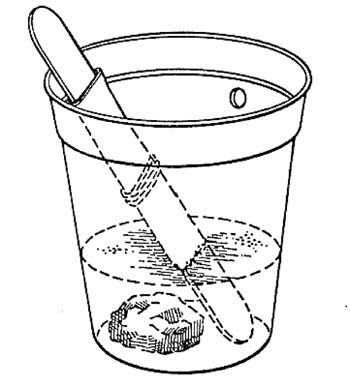
\includegraphics[width=6cm]{../book/capitulo-3/graphics/ovitrampa.jpg}
  \end{center}
\end{frame}

\begin{frame}[c]{Strack tecnológico.}
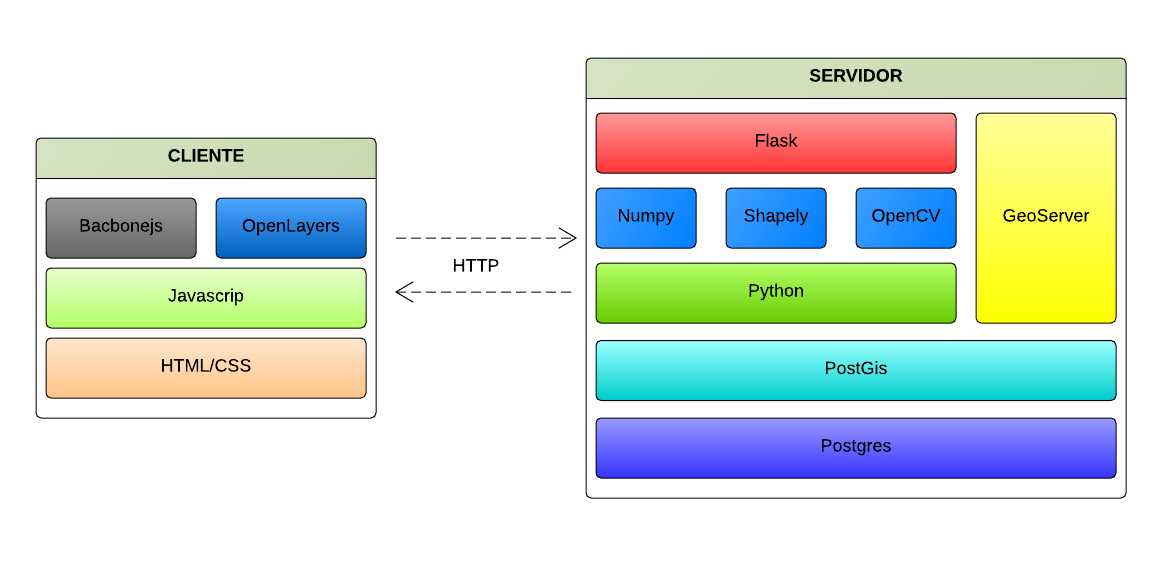
\includegraphics[width=\textwidth]{../book/capitulo-5/graphics/stack-tecnologias.png}
\end{frame}


\begin{frame}[c]{Conteo de larvas con PDI.}
    \begin{figure}
    \begin{subfigure}[b]{0.45\textwidth}
        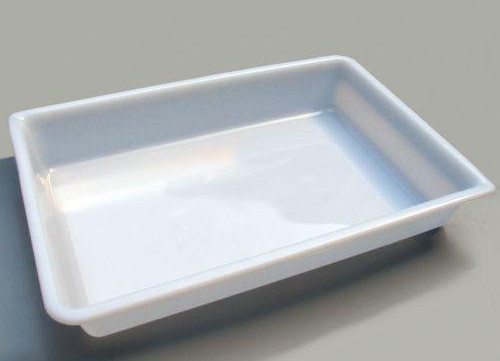
\includegraphics[width=4.5cm]{../book/capitulo-5/graphics/bandeja-muestra.jpg}
        \caption{Bandeja vacía.}
    \end{subfigure}
    ~~~~
    \begin{subfigure}[b]{0.45\textwidth}
        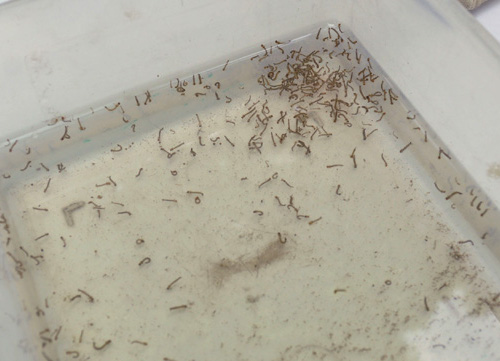
\includegraphics[width=4.5cm]{../book/capitulo-5/graphics/larvas-dengue.jpg}
        \caption{Bandeja con larvas.}
    \end{subfigure}
    \end{figure}
\end{frame}

\begin{frame}[c]{Conteo de larvas con PDI (2).}
    \begin{figure}
    \begin{subfigure}[t]{0.45\textwidth}
        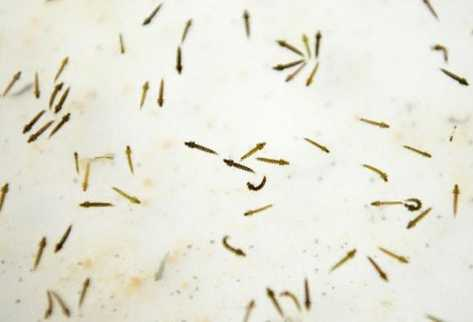
\includegraphics[width=4.5cm]{../book/capitulo-5/graphics/larvas-original.png}
        \caption{Imagen original.}
    \end{subfigure}
    ~~~~
    \begin{subfigure}[t]{0.45\textwidth}
        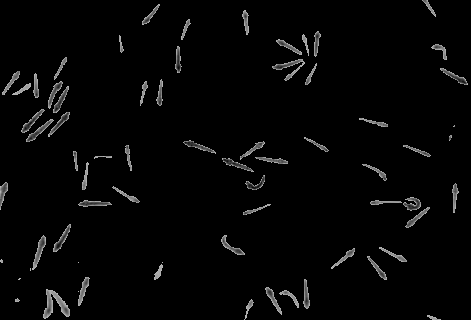
\includegraphics[width=4.5cm]{../book/capitulo-5/graphics/larvas-otsu.png}
        \caption{Imagen luego de la umbralización.}
    \end{subfigure}
    \end{figure}
\end{frame}

\begin{frame}[t]{Interpolación Espacial.}
  \begin{center}
   \begin{columns}[T]
        \begin{column}[T]{3.5cm}
            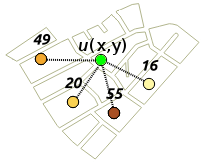
\includegraphics[width=4cm]{./graphics/interpolacion-ej.png}
        \end{column}
        \begin{column}[T]{7cm}
        \begin{equation}\label{eq:interpolacion-idw}
         u(x,y) = \sum_{i=1}^{N} w_i(x,y) * u_{i}
        \end{equation}
        Donde :
        \begin{equation}
        w_i(X) =  \dfrac{d((x,y), (x_i,y_i))^{-p}}{\sum_{j=1}^{N} d((x,y), (x_j,y_j))^{-p}}
        \end{equation}
        \end{column}
    \end{columns}
  \end{center}
    \text{Ejemplo:}
    $u(x,y) = w_1(x,y) * 49 + w_2(x,y) * 20 + w_3(x,y) * 55 + w_4(x,y) * 16 $
\end{frame}

{
\usebackgroundtemplate{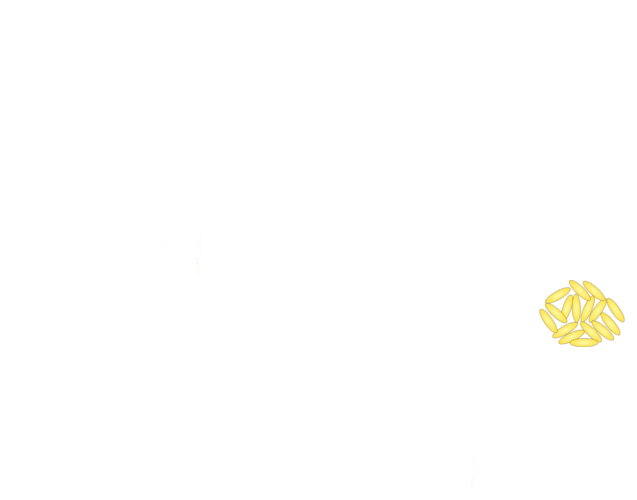
\includegraphics[width=\paperwidth]{./graphics/huevos.png}}
\begin{frame}[c]{Modelos de simulación de la ecología del vector.\\\textit{Mortalidad de los huevos(Otero et al., 2006).}}
  % poseen una gran resistencia
  \begin{center}
      \begin{equation}
          M_{H(x,y)} = me * H(x,y)
      \end{equation}
  \end{center}
  Donde :
    \begin{itemize}
      \item $me$ : Tasa de mortalidad diaria igual a $0,01\  \text{días}^{-1}$.
      \item $H(x, y)$ : Cantidad de huevos observados en $(x,y)$.
      \item $M_{H(x,y)}$ : Cantidad de huevos a eliminar.
    \end{itemize}
\end{frame}
}

{
\usebackgroundtemplate{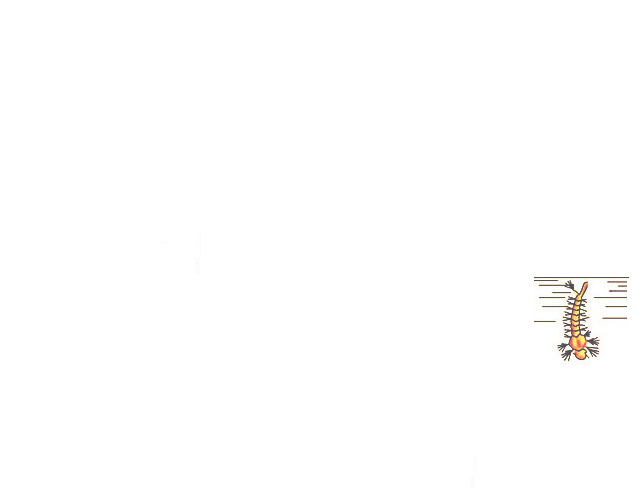
\includegraphics[width=\paperwidth]{./graphics/larva.png}}
\begin{frame}[c]{Simulación del proceso evolutivo. \\\textit{Mortalidad de larvas (Otero et al., 2006)}}
  Mortalidad bajo óptimas condiciones de las larvas:
  \begin{center}
    \begin{equation}
    \label{eq:mortalidad-natural-larvas}
        ml(k) = 0.01 + 0.9725 * exp\bigg( \frac{-(k - 278)}{2.7035}\bigg)
    \end{equation}
  \end{center}
  Donde :
    \begin{itemize}
      \item $k$ : Temperatura en Kelvin.
    \end{itemize}
\end{frame}

\begin{frame}[c]{Modelos de simulación de la ecología del vector.\\\textit{Mortalidad de larvas (Otero et al., 2006).}}
  \begin{center}
      \begin{equation}
      M_{L(x,y)}(k) = ml(k) * L(x,y) + \bigg(\frac{\alpha _{0}}{BS(x,y)}\bigg) * L(x,y) *(L(x,y) - 1)
    \end{equation}
  \end{center}
  Donde:
 \begin{itemize}
      \item $k$ : Temperatura en Kelvin.
      \item $L(x, y)$ : Cantidad de larvas observadas en $(x,y)$.
      \item $\alpha _{0}$ : Capacidad de carga de un solo lugar de reproducción.
      \item $BS(x,y)$ : Es el número de sitios de reproducción en $(x,y)$ .
      \item $M_{L(x,y)}$ : Cantidad de larvas a eliminar.
    \end{itemize}
\end{frame}
}


{
\usebackgroundtemplate{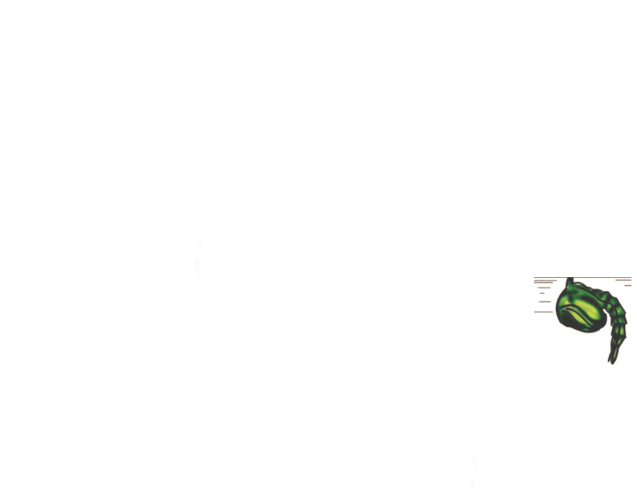
\includegraphics[width=\paperwidth]{./graphics/pupas.png}}

\begin{frame}[c]{Simulación del proceso evolutivo. \\\textit{Mortalidad de las pupas (Otero et al., 2006)}}
  Mortalidad bajo óptimas condiciones de la pupa:
  \begin{center}
    \begin{equation}
    \label{eq:mortalidad-natural-pupas}
        mp(k) = 0.01 + 0.9725 * exp\bigg( \frac{-(k - 278)}{2.7035}\bigg)
    \end{equation}
  \end{center}
  Donde :
    \begin{itemize}
      \item $k$ : Temperatura en Kelvin.
    \end{itemize}
\end{frame}

\begin{frame}[c]{Modelos de simulación de la ecología del vector.\\\textit{Mortalidad de las pupas (Otero et al., 2006).}}
  \begin{center}
    \begin{equation}
        M_{P(x,y)}(k) = P(x,y) * (mp(k) + (1 - ef) * R(k))
    \end{equation}
  \end{center}
  Donde :
    \begin{itemize}
      \item $k$ : Temperatura en Kelvin.
      \item $ef$ : El factor de supervivencia es de $0,83$.
      \item $R(k)$ : La tasa de desarrollo de la pupa.
      \item $P(x, y)$ : Cantidad de pupas observadas en $(x,y)$.
      \item $M_{P(x,y)}$ : Cantidad de pupas a eliminar.
    \end{itemize}
\end{frame}
}


{
\usebackgroundtemplate{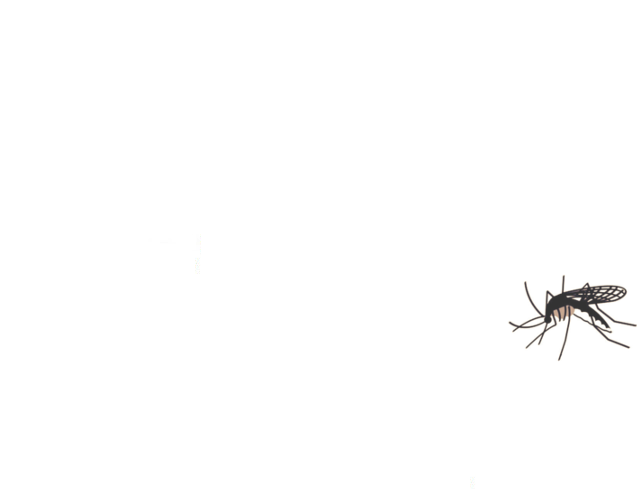
\includegraphics[width=\paperwidth]{./graphics/adulto.png}}
\begin{frame}[c]{Modelos de simulación de la ecología del vector.\\\textit{Mortalidad de adultos (Otero et al., 2006).}}
 % 10% diario, 50% semanal, 95% a final del primer mes.
  % Es constante, a pesar de su alta mortalidad, si la población
  % es lo sifucientemente grande, puede llegar a causar una epidemia
  \begin{center}
    \begin{equation}
        M_{A(x,y)} = ma * A(x,y)
    \end{equation}
  \end{center}
  Donde:
    \begin{itemize}
      \item $ma$ : Tasa de mortalidad diaria igual a $0,09$ \ $1/\text{días}$.
      \item $A(x, y)$ : Cantidad de adultos observados en $(x,y)$.
      \item $M_{A(x,y)}$ : Cantidad de adultos a eliminar.
    \end{itemize}
\end{frame}
}

\begin{frame}[t]{Coeficientes del modelo de Sharpe y DeMichele.}
    \begin{itemize}
      \item $\Delta H_{A}$ : Es la entalpía de activación de la reacción que es catalizada por la enzima ($cal\ mol^{-1}$).
      \item $\Delta H_{H}$ : es el cambio de entalpía asociado con la alta temperatura de la inactivación de la enzima ($cal\ mol^{-1}$).
      \item $T_{1/2}$ : es la temperatura cuando la mitad de la enzima se desactiva, a causa de la alta temperatura ($K$).
      \item $R$ : es la constante universal de los gases 1,987 $cal\ mol^{-1}$ .
    \end{itemize}
\end{frame}

\begin{frame}[c]{Entalpía.}
 $\Delta H$ es cantidad de energía absorbida o cedida por un sistema termodinámico, es decir, la cantidad de energía que un sistema intercambia con su entorno.
    \begin{center}
        \begin{equation}
            \Delta H = H_{final} - H_{inicial}
        \end{equation}
    \end{center}
    Donde:
    \begin{itemize}
      \item $H_{final}$ :En una reacción química es la entalpía de los productos.
      \item $H_{inicial}$ :En una reacción química es la entalpía de los reactivos.
    \end{itemize}
\end{frame}
\begin{frame}[c]{Reactivos y productos.}
Los reactivos son aquellos compuestos de una reacción química que combinados con otros compuestos, permiten obtener compuestos diferentes(productos). Los productos son el resultado de mezcla de los reactivos.
\begin{center}
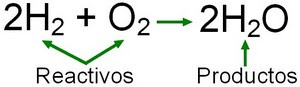
\includegraphics[width=7cm]{./graphics/reactivos-productos.jpg}
\end{center}
\end{frame}

\begin{frame}[t]{Coeficientes del modelo de Sharpe y DeMichele.}
\begin{table}
\begin{minipage}{\textwidth}
    \centering
    \small
    \caption{ \label{tab:coef-sharpe-demichele} Coeficientes para el modelo simplificado de Sharpe y DeMichele, con inhibición de altas temperaturas presentado por Schoolfield.}
    \begin{tabular}{l c r r r r }
        \hline \\
        Ciclo de desarrollo    & $R(298K)$ & $\Delta H_{A}$ & $\Delta H_{H}$ & $\Delta T_{1/2}$  \\
        \hline
        \hline
        Eclosión de los huevos$^a$ & 0,24000 & 10798,00 &  100000,00  & 14184,000\\
        Desarrollo larvario$^b$    & 0,20429 & 36072,78 &   59147,51  &   301,560\\
        Desarrollo pupal$^b$       & 0,74423 & 19246,42 &    5954,35  &   302,687\\
        Ciclo gonotrófico (AN)$^c$ & 0,21600 & 15725,00 & 1756481,00  &   447,200\\
        Ciclo gonotrófico (AP)$^c$ & 0,37200 & 15725,00 & 1756481,00  &   447,200\\
    \end{tabular}
    \footnotetext[1]{Coeficientes Otero et al., 2006.}
    \footnotetext[2]{Coeficientes Rueda et al.,1990.}
    \footnotetext[3]{Coeficientes, para AP y AN, tomados Otero et al., 2006.}
\end{minipage}
\end{table}
\end{frame}


\begin{frame}[t]{Mapas de interpolación a 20 \textcelsius.}
    \begin{figure}
    \begin{subfigure}[b]{0.45\textwidth}
        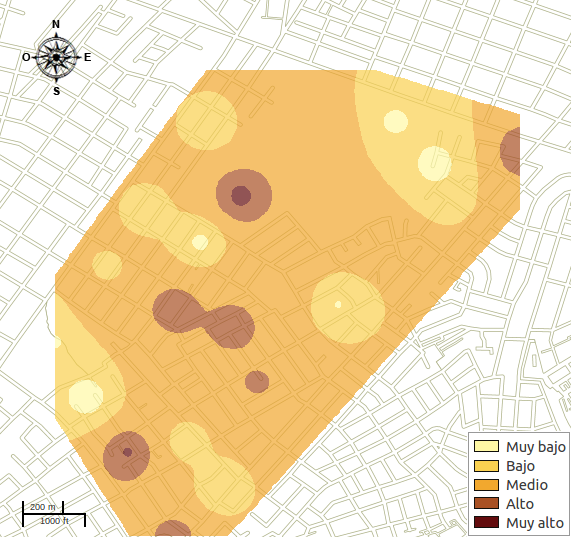
\includegraphics[width=\textwidth]{../book/capitulo-6/graphics/raster/temp-20-0.png}
        \caption{ Primer día de simulación.}
    \end{subfigure}
    ~~~~
    \begin{subfigure}[b]{0.45\textwidth}
        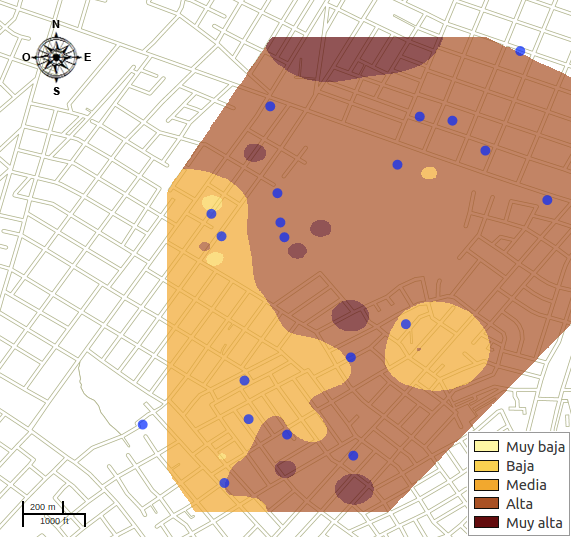
\includegraphics[width=\textwidth]{../book/capitulo-6/graphics/raster/temp-20-38.png}
        \caption{Día número 50 de simulación.}
    \end{subfigure}
    \end{figure}
\end{frame}

\begin{frame}[t]{Mapas de interpolación a 24 \textcelsius.}
    \begin{figure}
    \begin{subfigure}[b]{0.45\textwidth}
        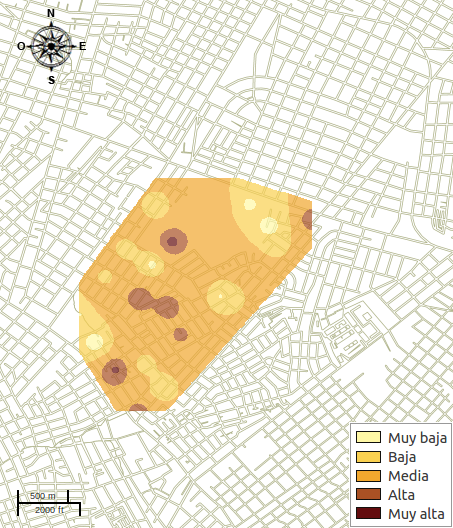
\includegraphics[width=4.5cm]{../book/capitulo-6/graphics/raster/temp-24-0.png}
        \caption{ Primer día de simulación.}
    \end{subfigure}
    ~~~~
    \begin{subfigure}[b]{0.45\textwidth}
        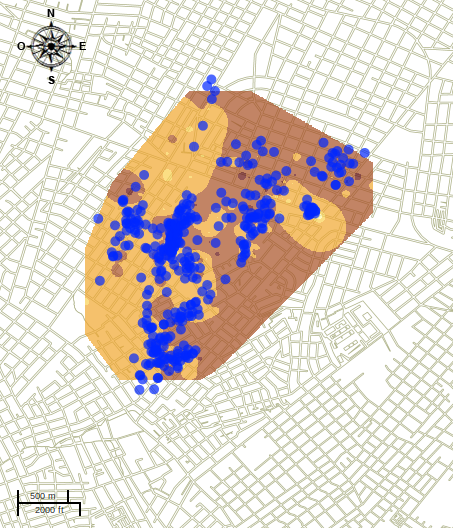
\includegraphics[width=4.5cm]{../book/capitulo-6/graphics/raster/temp-24-49.png}
        \caption{Día número 50 de simulación.}
    \end{subfigure}
    \end{figure}
\end{frame}

\begin{frame}[t]{Mapas de interpolación a 27 \textcelsius.}
    \begin{figure}
    \begin{subfigure}[b]{0.45\textwidth}
        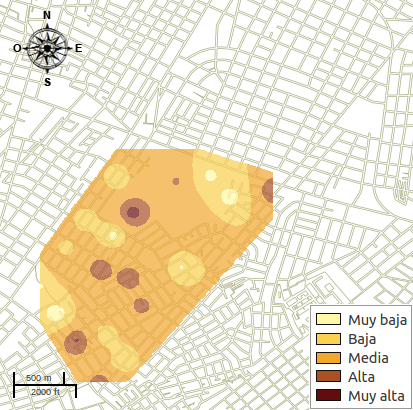
\includegraphics[width=\textwidth]{../book/capitulo-6/graphics/raster/temp-27-0.png}
        \caption{ Primer día de simulación.}
    \end{subfigure}
    ~~~~
    \begin{subfigure}[b]{0.45\textwidth}
        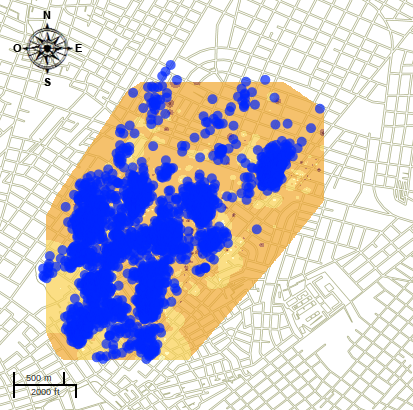
\includegraphics[width=\textwidth]{../book/capitulo-6/graphics/raster/temp-27-49.png}
        \caption{Día número 50 de simulación}
    \end{subfigure}
    \end{figure}
\end{frame}

\begin{frame}[t]{Mapas de interpolación a 34 \textcelsius.}
    \begin{figure}
    \begin{subfigure}[b]{0.45\textwidth}
        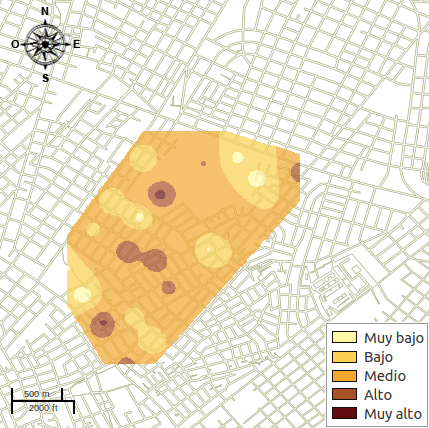
\includegraphics[width=\textwidth]{../book/capitulo-6/graphics/raster/temp-34-0.png}
        \caption{ Primer día de simulación.}
    \end{subfigure}
    ~~~~
    \begin{subfigure}[b]{0.45\textwidth}
        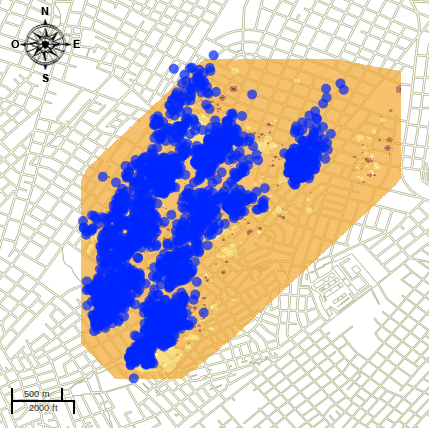
\includegraphics[width=\textwidth]{../book/capitulo-6/graphics/raster/temp-34-42.png}
        \caption{Día número 50 de simulación.}
    \end{subfigure}
    \end{figure}
\end{frame}


